\documentclass{article}

\usepackage[preprint]{neurips_2026}

\usepackage[utf8]{inputenc}
\usepackage[T1]{fontenc}
\usepackage{hyperref}
\usepackage{url}
\usepackage{booktabs}
\usepackage{amsfonts}
\usepackage{amsmath}
\usepackage{microtype}
\usepackage{xcolor}
\usepackage{graphicx}
\usepackage{siunitx}

\title{Comparing 2D, 2.5D, and 3D Residual U-Nets for T1 MRI Denoising}

\author{%
  Computational Neuroscience Final Project\\
  T1 MRI Denoising Task\\
  \texttt{T1\_noisy.nii.gz} $\rightarrow$ \texttt{T1\_clean.nii.gz}
}

\begin{document}

\maketitle

\begin{abstract}
This project studies supervised denoising of paired T1-weighted MRI volumes. Each case provides a noisy T1 image and a clean target image from the same subject, allowing direct training and evaluation with image restoration metrics. We compare three residual U-Net variants: a 2D slice model, a 2.5D model that uses adjacent axial slices as input channels, and a patch-based 3D model. All methods are trained on the same 600-case dataset with case-level train, validation, and test splits. On the held-out test set, every learned model improves over the noisy input. Under a unified 48-slice-per-case evaluation protocol, the best result is obtained by the 2.5D Residual U-Net, which reduces MAE from 0.0044 to 0.0027, improves PSNR from 44.7988 dB to 47.8719 dB, and improves SSIM from 0.9552 to 0.9950. The results suggest that a small amount of through-plane context is useful for this task, while the 3D patch baseline is harder to optimize under the available training budget.
\end{abstract}

\section{Introduction}

MRI denoising is a standard image restoration problem: given a noisy image $x$ and a clean target image $y$, the goal is to learn a mapping $f_\theta(x)$ that suppresses noise while preserving anatomical structure. This project uses the denoising option from the course final task because the input and target belong to the same modality and are spatially paired, which makes supervised training and quantitative evaluation straightforward.

U-Net models are widely used in biomedical image analysis because encoder-decoder paths capture multi-scale context while skip connections preserve local detail \citep{Ronneberger2015UNet}. Volumetric U-Nets extend the same idea to 3D data \citep{Cicek20163DUNet}. In denoising, residual prediction is a natural design choice: the noisy and clean images share most anatomy, so the network only needs to learn a correction term. We therefore compare 2D, 2.5D, and 3D residual U-Net baselines on the same T1 MRI denoising task.

\section{Data}

The data root is \texttt{data/cn\_project\_t1\_noise2}. Each case directory contains \texttt{T1\_noisy.nii.gz} and \texttt{T1\_clean.nii.gz}. The experiment uses 600 complete paired cases. We split data at the case level with random seed 42, producing 420 training cases, 90 validation cases, and 90 test cases. Case-level splitting avoids leakage from putting slices of the same subject into different splits.

\section{Methods}

\subsection{Preprocessing}

For each case, noisy and clean NIfTI volumes are loaded as 3D arrays. Intensities are normalized per case by computing the 1st and 99th percentiles over the joint foreground voxels from noisy and clean images, then clipping and scaling values to $[0,1]$. Near-empty axial slices are skipped. For 2D and 2.5D models, slices are resized to $256\times256$. For the 3D model, training uses cropped volumetric patches.

\subsection{Residual U-Net Variants}

The 2D model takes one axial slice as input and predicts the denoised version of the same slice. The 2.5D model uses three adjacent axial slices, $(z-1,z,z+1)$, as input channels and predicts the clean center slice. This gives the network limited through-plane context while keeping the cheaper 2D convolutional architecture. The 3D model uses 3D convolutions and is trained on volumetric patches of size $32\times96\times96$ in depth, height, and width.

All models predict a residual correction. For 2D and 2.5D, the output is
\begin{equation}
  \hat{y} = \mathrm{clip}(x_c + r_\theta(x), 0, 1),
\end{equation}
where $x_c$ is the input slice for 2D and the center slice for 2.5D. For 3D, the residual is added to the input patch. The final residual layer is zero-initialized so the initial network behaves like the noisy baseline.

\subsection{Training}

The loss combines L1 and MSE terms:
\begin{equation}
  \mathcal{L}(\hat{y}, y) =
  \|\hat{y}-y\|_1 + 0.2\|\hat{y}-y\|_2^2.
\end{equation}
All models use AdamW \citep{Kingma2015Adam} with learning rate $10^{-4}$ and weight decay $10^{-5}$. The 2D model is trained for 40 epochs with batch size 24. The 2.5D model is trained with the same learning rate and early stopping, selecting the best checkpoint at epoch 8. The 3D model is trained as a patch-based baseline with smaller batch size because volumetric convolutions require more memory.

\section{Evaluation}

We evaluate on the 90 held-out test cases using MAE, MSE, PSNR, and SSIM \citep{Wang2004SSIM}. MAE and MSE are lower-is-better; PSNR and SSIM are higher-is-better. Metrics are computed per case and then averaged across cases. To make the three methods directly comparable, all reported results use the same 48 uniformly sampled valid slices per test case.

\section{Results}

\subsection{Training Behavior}

The 2D model reaches its best validation loss at epoch 36. The 2.5D model reaches its best validation loss at epoch 8 and then early-stops at epoch 14. The 3D patch model improves during its short run, but remains harder to optimize because each update sees fewer full anatomical contexts than the slice-based models.

\begin{figure}[h]
  \centering
  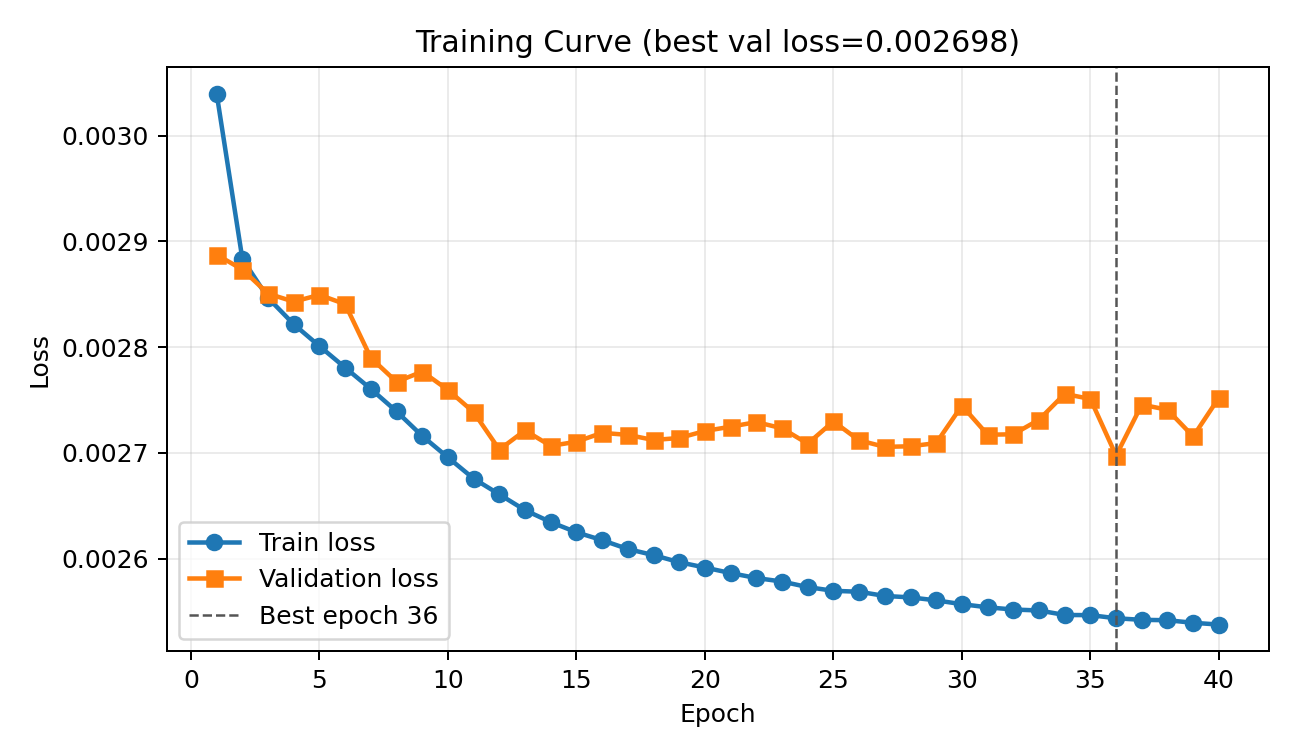
\includegraphics[width=0.32\linewidth]{figures/curves/training_2d.png}
  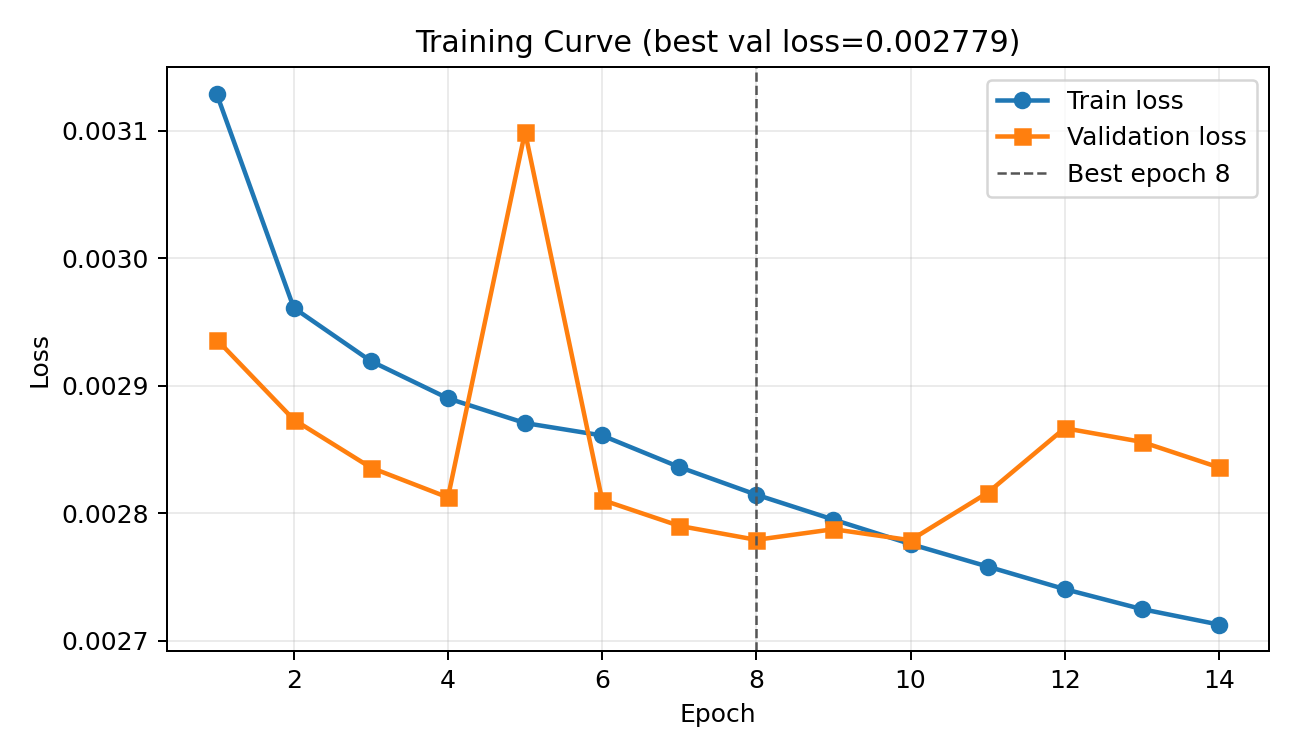
\includegraphics[width=0.32\linewidth]{figures/curves/training_25d.png}
  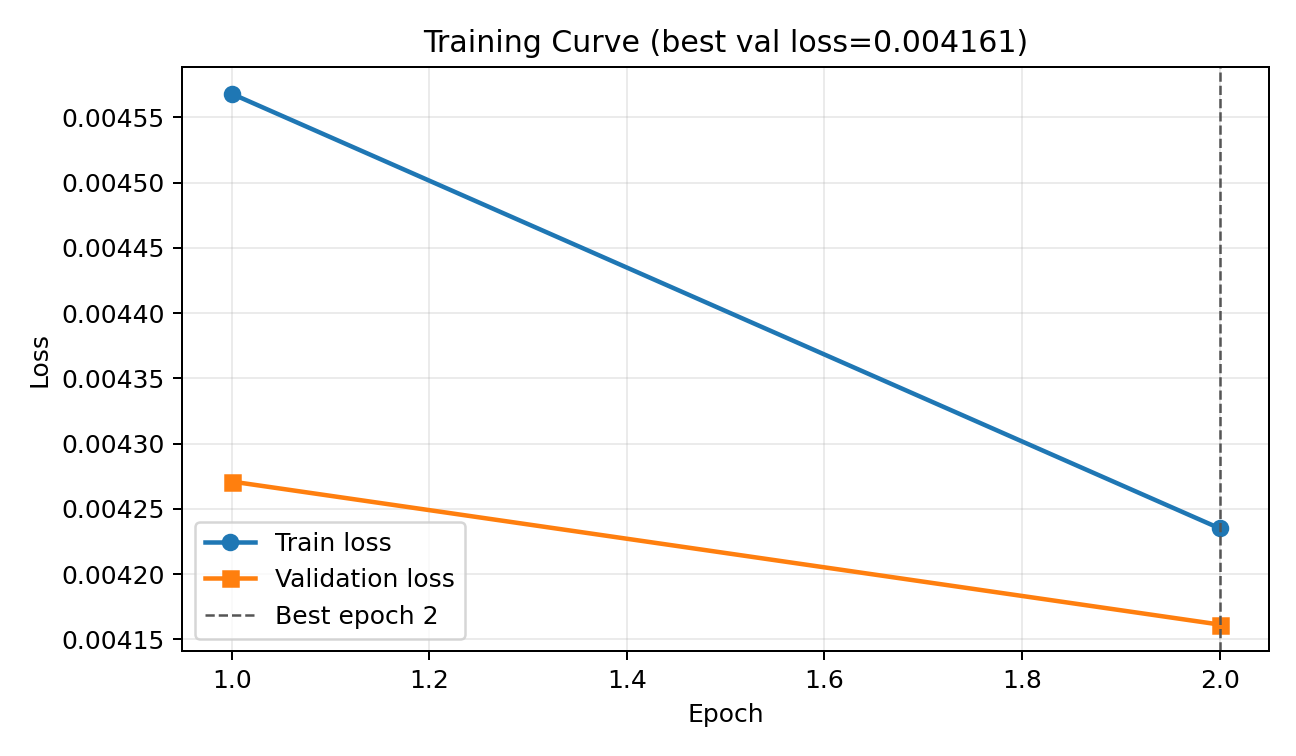
\includegraphics[width=0.32\linewidth]{figures/curves/training_3d.png}
  \caption{Training and validation loss curves for the 2D, 2.5D, and 3D residual U-Net variants.}
  \label{fig:training_curves}
\end{figure}

\subsection{Quantitative Comparison}

Table~\ref{tab:summary} summarizes the test-set results. The 2.5D model gives the strongest numerical result among the implemented methods. It slightly improves over the 2D model, which suggests that adjacent slices provide useful context. The 3D model still improves over the noisy input, but it does not outperform the slice-based models under the current patch-based training and evaluation budget.

\begin{table}[h]
  \centering
  \caption{Case-level mean metrics on the 90-case test set.}
  \label{tab:summary}
  \begin{tabular}{lrrrr}
    \toprule
    Method & MAE $\downarrow$ & MSE $\downarrow$ & PSNR $\uparrow$ & SSIM $\uparrow$ \\
    \midrule
    Noisy baseline & 0.0044 & $3.70\times10^{-5}$ & 44.7988 & 0.9552 \\
    2D Residual U-Net & 0.0028 & $1.79\times10^{-5}$ & 47.7427 & 0.9949 \\
    2.5D Residual U-Net & \textbf{0.0027} & $\mathbf{1.74\times10^{-5}}$ & \textbf{47.8719} & \textbf{0.9950} \\
    3D Residual U-Net & 0.0030 & $2.00\times10^{-5}$ & 47.2754 & 0.9912 \\
    \bottomrule
  \end{tabular}
\end{table}

\subsection{Qualitative Results}

Figure~\ref{fig:qualitative} shows representative 2.5D outputs. The denoised images are visually closer to the clean targets than the noisy inputs, and the absolute error maps are weaker after denoising.

\begin{figure}[h]
  \centering
  
\includegraphics[width=\linewidth]{figures/25d/1000542.png}
  
\includegraphics[width=\linewidth]{figures/25d/1002722.png}
  
\includegraphics[width=\linewidth]{figures/25d/1002807.png}
  \caption{Qualitative results for three held-out test cases using the 2.5D Residual U-Net. In each row, the columns are Noisy, Denoised, Clean, and Absolute Error.}
  \label{fig:qualitative}
\end{figure}

\section{Discussion}

All three residual U-Net variants improve the noisy input, which indicates that the paired denoising task is well suited to supervised residual learning. The comparison between 2D and 2.5D is especially informative. Adding the neighboring axial slices gives the network limited anatomical context across the slice direction, but it does not substantially increase model complexity because the convolutions remain two-dimensional. This likely explains why the 2.5D model achieves the best PSNR and SSIM while staying close to the computational cost of the 2D baseline.

The 3D model also improves the noisy baseline, but its advantage is not visible under the current setting. This does not necessarily mean that volumetric modeling is unhelpful for MRI denoising. In this experiment, the 3D U-Net is trained on patches to fit memory constraints, and evaluation predicts center slices from a fixed depth window rather than reconstructing full volumes with dense overlap. These choices make the experiment feasible on the available hardware, but they reduce the amount of global context used by the model and make optimization more difficult. With longer training, more patch samples per case, and overlap-averaged sliding-window inference, a 3D model may become more competitive.

\section{Conclusion}

This project implements and compares 2D, 2.5D, and 3D residual U-Nets for supervised T1 MRI denoising. On the 600-case dataset with 90 held-out test cases, all learned models improve over the noisy baseline. The 2.5D model performs best among the implemented variants, showing that adjacent-slice context is a good trade-off between accuracy and implementation complexity for this course project.

\section*{Code Availability}

The code and report files are available at \url{https://github.com/liuxiangyu666777888/Computational_Neurobiology}.

\bibliographystyle{plainnat}
\bibliography{references}

\end{document}
